\documentclass[tikz]{standalone}
\usepackage[utf8]{inputenc}

\begin{document}

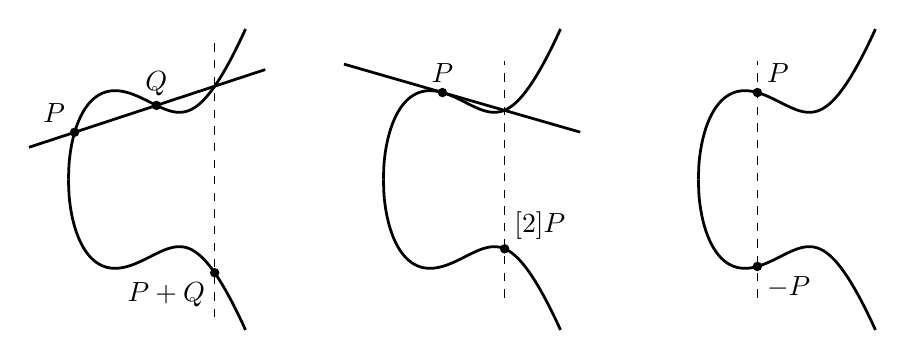
\begin{tikzpicture}[scale=.5]
\draw[domain=-2:2.5,smooth,samples=300,line width=1pt] plot (\x, {sqrt(\x^3 - 2*\x + 4)});
\draw[domain=-2:2.5, smooth, samples=300, line width=1pt] plot (\x, {- sqrt(\x^3 - 2*\x + 4)});
\fill (-1.842,1.2) circle (0.12) node[above left] {$P$};
\fill (0.235,1.882) circle (0.12) node[above] {$Q$};
\fill (1.715,-2.37) circle (0.12) node[below left] {$P+Q$};
\draw[domain=-3:3, smooth, samples=300, line width=1pt] plot (\x, {.329*\x + 1.805});
\draw[dashed] (1.715, -3.5) -- (1.715, 3.5);

\begin{scope}[shift={(8,0)}]
\draw[domain=-2:2.5, smooth, samples=300, line width=1pt] plot (\x, {sqrt(\x^3 - 2*\x + 4)}) ;
\draw[domain=-2:2.5, smooth, samples=300, line width=1pt] plot (\x, {- sqrt(\x^3 - 2*\x + 4)});
\fill (-.5,2.208) circle (.12) node[above] {$P$};
\fill (1.08, -1.761) circle (.12) node[above right] {$[2]P$};
\draw[domain=-3:3, smooth, samples=300, line width=1pt] plot (\x, {-.288*\x + 2.066});
\draw[dashed] (1.08, -3) -- (1.08, 3);
\end{scope}

\begin{scope}[shift={(16,0)}]
\draw[domain=-2:2.5, smooth, samples=300, line width=1pt] plot (\x, {sqrt(\x^3 - 2*\x + 4)}) ;
\draw[domain=-2:2.5, smooth, samples=300, line width=1pt] plot (\x, {- sqrt(\x^3 - 2*\x + 4)});
\fill (-.5,2.208) circle (.12) node[above right] {$P$};
\fill (-.5,-2.208) circle (.12) node[below right] {$-P$};
\draw[dashed] (-.5, -3) -- (-.5, 3);
\end{scope}
\end{tikzpicture}

\end{document}